\documentclass[12pt,a4paper]{article}

% --- Настройка языка и шрифтов для LuaLaTeX ---
\usepackage{fontspec}
\defaultfontfeatures{Ligatures=TeX,Scale=MatchLowercase}

\setmainfont{Alice-Regular}[
    Path=font/,
    Extension=.ttf,
    BoldFont = Alice-Regular,
    ItalicFont = Alice-Regular,
    BoldItalicFont = Alice-Regular,
    BoldFeatures = {FakeBold=1.6},
    ItalicFeatures = {FakeSlant=0.2},
    BoldItalicFeatures = {FakeBold=1.6,FakeSlant=0.2}
]

\newfontfamily\cyrillicfont{Alice-Regular}[
    Path=font/,
    Extension=.ttf,
    BoldFont = Alice-Regular,
    ItalicFont = Alice-Regular,
    BoldItalicFont = Alice-Regular,
    BoldFeatures = {FakeBold=1.6},
    ItalicFeatures = {FakeSlant=0.2},
    BoldItalicFeatures = {FakeBold=1.6,FakeSlant=0.2}
]

\usepackage{polyglossia}
\setmainlanguage{russian}
\setsansfont{TeX Gyre Heros}
\setmonofont{TeX Gyre Cursor}

\usepackage{graphicx}        					          % Графика
\usepackage[protrusion=false]{microtype}       	% Микротипографика
\usepackage{amsmath, amsfonts, amssymb, amsthm}	% Математика
\usepackage{braket} 							              % Braket нотация для квантовой механики
\usepackage{unicode-math} 						          % Современный пакет для математики в LuaLaTeX
\usepackage{longtable}       					          % Таблицы с разрывом страниц
\usepackage{tikz}           					          % Рисование
\usepackage[europeanresistors]{circuitikz}		  % Рисование электрических схем в европейском стиле
\usepackage{listings}							              % Для отображения кода
\usepackage{tabularx}       					          % Для таблиц во всю ширину
\usepackage{array}		  						            % Для расширенных возможностей таблиц
\usepackage{float}          					          % Для точного позиционирования фигур
\usepackage{pgfplots}                           % Для построения графиков
\usepackage{caption}                            % Для настройки подписей к рисункам и таблицам
\usepackage{xfp}                                % Для вычислений в LaTeX
\pgfplotsset{compat=1.18}
\usepackage[a4paper,left=20mm,right=20mm,top=20mm,bottom=20mm]{geometry}

\usetikzlibrary{arrows.meta}

% --- Колонтитулы ---
\usepackage{fancyhdr}
\pagestyle{fancy}
\fancyhf{}

\renewcommand{\headrulewidth}{0.4pt}
\renewcommand{\footrulewidth}{0.4pt}
\renewcommand\lstlistingname{Исходный код}

\lstdefinestyle{main}{
	backgroundcolor=\color{gray!8},   
	commentstyle=\color{green!50!black},
	keywordstyle=\color{blue!80!black},
	numberstyle=\small\color{darkgray},
	stringstyle=\rmfamily\color{orange!90!black},
	basicstyle=\ttfamily\small,
	breakatwhitespace=false,         
	breaklines=true,                   
	keepspaces=true,                 
	numbers=left,                    
	numbersep=8pt,                  
	showspaces=false,                
	showstringspaces=false,
	showtabs=false,                  
	tabsize=4
}	

\lstset{style=main}

\newcolumntype{C}{>{\centering\arraybackslash}X}
\renewcommand{\arraystretch}{1.25}

% =========================================================
%         СЛУЖЕБНЫЕ КОМАНДЫ ДЛЯ ВЫЧИСЛЕНИЙ
% =========================================================
\newcommand{\CalcZero} [1]{\fpeval{round((#1),0)}}
\newcommand{\CalcOne}  [1]{\fpeval{round((#1),1)}}
\newcommand{\CalcTwo}  [1]{\fpeval{round((#1),2)}}
\newcommand{\CalcThree}[1]{\fpeval{round((#1),3)}}
\newcommand{\CalcFour} [1]{\fpeval{round((#1),4)}}
\newcommand{\CalcFive} [1]{\fpeval{round((#1),5)}}

% ---------------------------------------------------------
% ОБЩИЕ ДАННЫЕ
% ---------------------------------------------------------
\def\VariantN{1}          					         % Номер варианта
\def\StudentName{Андреев Иван Алексеевич}  	 % ФИО студента
\def\TeacherName{Устинов Юрий Александрович} % ФИО преподавателя
\def\LabNumber{3}							               % Номер лабораторной работы
\def\Discipline{Электроника}				           % Название дисциплины
\def\LabTitle{Исследование усилительного каскада с ёмкостной связью}	 % Название лабораторной работы

\def\Uone{\CalcTwo{5 + (\VariantN)^(1/4)}} % Напряжение питания
\def\Ub  {1.548} % напряжение эмиттера
\def\Ue  {\fpeval{972.443 * 10^(-3)}} % напряжение база-эмиттер
\def\Ube {\fpeval{\Ub - \Ue}} % напряжение база-эмиттер
\def\Ik  {\fpeval{648.22 * 10^(-6)}} % эмиттерный ток
\def\Uke {\fpeval{\Uone - \Ik * 3300 - \Ue}} % напряжение коллектор-эмиттер

\def\IkTwenty{\Ik} % эмиттерный ток для 20% R6
\def\IkThirty{\fpeval{614.008 * 10^(-6)}} % эмиттерный ток для 30% R6
\def\IkForty{\fpeval{577.974 * 10^(-6)}} % эмиттерный ток для 40% R6
\def\IkFifty{\fpeval{539.991 * 10^(-6)}} % эмиттерный ток для 50% R6
\def\IkSixty{\fpeval{499.931 * 10^(-6)}} % эмиттерный ток для 60% R6
\def\IkSeventy{\fpeval{457.644 * 10^(-6)}} % эмиттерный ток для 70% R6
\def\IkEighty{\fpeval{413.017 * 10^(-6)}} % эмиттерный ток для 80% R6
\def\IkNinety{\fpeval{365.912 * 10^(-6)}} % эмиттерный ток для 90% R6
\def\IkHundred{\fpeval{316.232 * 10^(-6)}} % эмиттерный ток для 100% R6

\def\UeTwenty{\Ue} % напряжение база-эмиттер для 20% R6
\def\UeThirty{\fpeval{921.116 * 10^(-3)}} % напряжение база-эмиттер для 30% R6
\def\UeForty{\fpeval{867.057 * 10^(-3)}} % напряжение база-эмиттер для 40% R6
\def\UeFifty{\fpeval{810.077 * 10^(-3)}} % напряжение база-эмиттер для 50% R6
\def\UeSixty{\fpeval{749.981 * 10^(-3)}} % напряжение база-эмиттер для 60% R6
\def\UeSeventy{\fpeval{686.558 * 10^(-3)}} % напряжение база-эмиттер для 70% R6
\def\UeEighty{\fpeval{619.607 * 10^(-3)}} % напряжение база-эмиттер для 80% R6
\def\UeNinety{\fpeval{548.940 * 10^(-3)}} % напряжение база-эмиттер для 90% R6
\def\UeHundred{\fpeval{474.406 * 10^(-3)}} % напряжение база-эмиттер для 100% R6

\def\UpTwenty{\fpeval{\Uone - \UeTwenty}} % напряжение коллектор-эмиттер для 20% R6
\def\UpThirty{\fpeval{\Uone - \UeThirty}} % напряжение коллектор-эмиттер для 30% R6
\def\UpForty{\fpeval{\Uone - \UeForty}} % напряжение коллектор-эмиттер для 40% R6
\def\UpFifty{\fpeval{\Uone - \UeFifty}} % напряжение коллектор-эмиттер для 50% R6
\def\UpSixty{\fpeval{\Uone - \UeSixty}} % напряжение коллектор-эмиттер для 60% R6
\def\UpSeventy{\fpeval{\Uone - \UeSeventy}} % напряжение коллектор-эмиттер для 70% R6
\def\UpEighty{\fpeval{\Uone - \UeEighty}} % напряжение коллектор-эмиттер для 80% R6
\def\UpNinety{\fpeval{\Uone - \UeNinety}} % напряжение коллектор-эмиттер для 90% R6
\def\UpHundred{\fpeval{\Uone - \UeHundred}} % напряжение коллектор-эмиттер для 100% R6

\def\Rfive{\fpeval{20 * 10^3 * 0.642}} % сопротивление резистора R5 для рабочей точки

\def\EgOne{\fpeval{2 * 10^{-3}}} % амплитудное значение генератора
\def\EgTwo{\fpeval{5 * 10^{-3}}} 
\def\EgThree{\fpeval{10 * 10^{-3}}}
\def\EgFour{\fpeval{15 * 10^{-3}}}
\def\EgFive{\fpeval{20 * 10^{-3}}}
\def\EgSix{\fpeval{25 * 10^{-3}}}
\def\EgSeven{\fpeval{30 * 10^{-3}}}
\def\EgEight{\fpeval{50 * 10^{-3}}}
\def\EgNine{\fpeval{80 * 10^{-3}}}
\def\EgTen{\fpeval{100 * 10^{-3}}}

\def\egOne  {\fpeval{1.414 * 10^(-3)}} % действующее значение генератора
\def\egTwo  {\fpeval{3.535 * 10^(-3)}}
\def\egThree{\fpeval{7.071 * 10^(-3)}}
\def\egFour {\fpeval{10.606 * 10^(-3)}}
\def\egFive {\fpeval{14.142 * 10^(-3)}}
\def\egSix  {\fpeval{17.678 * 10^(-3)}}
\def\egSeven{\fpeval{21.213 * 10^(-3)}}
\def\egEight{\fpeval{35.355 * 10^(-3)}}
\def\egNine {\fpeval{56.568 * 10^(-3)}}
\def\egTen  {\fpeval{70.710 * 10^(-3)}}

\def\UinOne  {\fpeval{1.157 * 10^(-3)}} % входное напряжение
\def\UinTwo  {\fpeval{2.892 * 10^(-3)}}
\def\UinThree{\fpeval{5.789 * 10^(-3)}}
\def\UinFour {\fpeval{8.692 * 10^(-3)}}
\def\UinFive {\fpeval{11.606 * 10^(-3)}}
\def\UinSix  {\fpeval{14.534 * 10^(-3)}}
\def\UinSeven{\fpeval{17.479 * 10^(-3)}}
\def\UinEight{\fpeval{29.453 * 10^(-3)}}
\def\UinNine {\fpeval{48.027 * 10^(-3)}}
\def\UinTen  {\fpeval{60.567 * 10^(-3)}}

\def\UoutOnekOhmOne  {\fpeval{11.137 * 10^(-3)}} % выходное напряжение для нагрузки 1 кОм
\def\UoutOnekOhmTwo  {\fpeval{27.818 * 10^(-3)}}
\def\UoutOnekOhmThree{\fpeval{55.456 * 10^(-3)}}
\def\UoutOnekOhmFour {\fpeval{82.740 * 10^(-3)}}
\def\UoutOnekOhmFive {\fpeval{109.506 * 10^(-3)}}
\def\UoutOnekOhmSix  {\fpeval{135.611 * 10^(-3)}}
\def\UoutOnekOhmSeven{\fpeval{160.932 * 10^(-3)}}
\def\UoutOnekOhmEight{\fpeval{252.741 * 10^(-3)}}
\def\UoutOnekOhmNine {\fpeval{360.575 * 10^(-3)}}
\def\UoutOnekOhmTen  {\fpeval{415.861 * 10^(-3)}}

\def\UoutTenkOhmOne  {\fpeval{35.027 * 10^(-3)}} % выходное напряжение для нагрузки 10 кОм
\def\UoutTenkOhmTwo  {\fpeval{87.488 * 10^(-3)}}
\def\UoutTenkOhmThree{\fpeval{174.412 * 10^(-3)}}
\def\UoutTenkOhmFour {\fpeval{260.222 * 10^(-3)}}
\def\UoutTenkOhmFive {\fpeval{344.412 * 10^(-3)}}
\def\UoutTenkOhmSix  {\fpeval{426.528 * 10^(-3)}}
\def\UoutTenkOhmSeven{\fpeval{506.174* 10^(-3)}}
\def\UoutTenkOhmEight{\fpeval{794.868 * 10^(-3)}}
\def\UoutTenkOhmNine {\fpeval{1.133}}
\def\UoutTenkOhmTen  {\fpeval{1.305}}

\def\KvOne{17.927} % dB 
\def\KvTwo{17.921}
\def\KvThree{9.5}
\def\KvFour{27.88}
\def\KvFive{17.925}

\def\fdOne{9.456} % нижняя граничная частота 
\def\fdTwo{39.104}
\def\fdThree{8.385}
\def\fdFour{5.101}
\def\fdFive{9.475}

\def\fuOne{\fpeval{1.545 * 10^6}} % верхняя граничная частота 
\def\fuTwo{\fpeval{1.556 * 10^6}}
\def\fuThree{\fpeval{425.959 * 10^3}}
\def\fuFour{\fpeval{604.662 * 10^3}}
\def\fuFive{\fpeval{51.218 * 10^3}}

\title{
	МИНОБРНАУКИ РОССИИ

	федеральное государственное автономное образовательное учреждение

	высшего образования

	«Национальный исследовательский университет
	«Московский институт электронной техники»
	\vspace{2em}
}
\author{
}
\date{}

\begin{document}

\maketitle
\thispagestyle{fancy}

\begin{center}
\Large Отчёт по Лабораторной работе $\LabNumber$\\
по дисциплине «\Discipline»\\
«\LabTitle»
\end{center}

\begin{center}
\Large Вариант \VariantN
\end{center}

\vspace{12em}

\begin{table}[h]
\noindent
\begin{tabular*}{\textwidth}{@{\extracolsep{\fill}} p{0.48\textwidth} p{0.52\textwidth}}
Студент, группа & \StudentName, ЭН-$25$ \\
[0.5em] Руководитель & \TeacherName
\end{tabular*}
\end{table}

\cfoot{Москва 2026}

\pagebreak

\fancyhead[L]{Задание $1$} 
\fancyhead[R]{\Discipline}
\fancyfoot[C]{\thepage}

\begin{figure}[H]
\centering
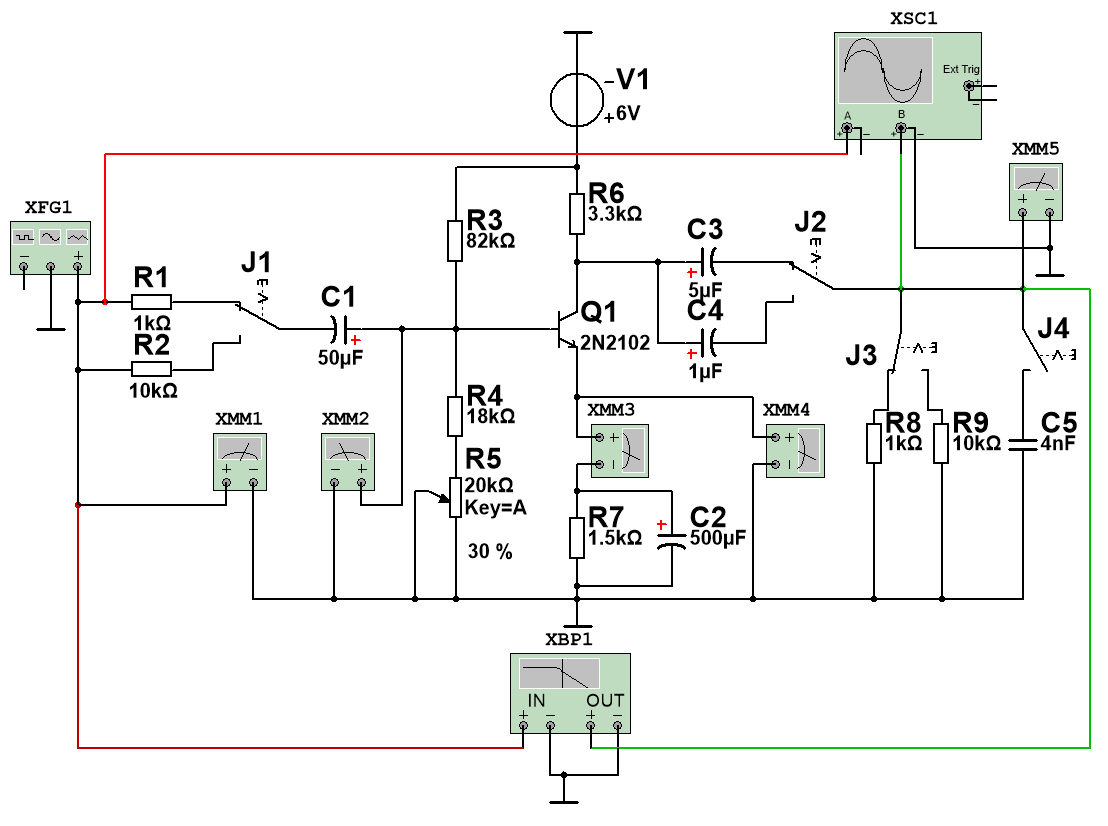
\includegraphics[width=\textwidth]{Exercise1.png}
\caption{Схема усилительного каскада}
\end{figure}

\begin{description}
	\item[V1]: согласно $\VariantN$-му варианту, напряжение питания $U_{V1} = 5 + \sqrt[4]{\VariantN} = \Uone$ В
	\item[R1]: входное сопротивления генератора $R_1 = 1$ кОм
	\item[R2]: входное сопротивления генератора $R_2 = 10$ кОм
	\item[J1]: переключатель входного сопротивления $R_1$ и $R_2$
	\item[R3]: резистор питания цепи базы $R_3 = 82$ кОм
	\item[R4]: резистор питания цепи базы $R_4 = 18$ кОм
	\item[R5]: переменный резистор питания цепи базы $R_5 = 20$ кОм
	\item[R6]: резистор питания цепи коллектора $R_6 = 3.3$ кОм  
	\item[R7]: резистор стабилизации эмиттера $R_7 = 1.5$ кОм
	\item[R8]: резистор активного сопротивления нагрузки $R_8 = 1$ кОм
	\item[R9]: резистор активного сопротивления нагрузки $R_9 = 10$ кОм
	\item[J3]: переключатель активного сопротивления нагрузки $R_8$ и $R_9$   
	\item[Q1]: биполярный транзистор $2$N$2102$, усилительный элемент
	\item[C1]: разделяющий конденсатор $C_1 = 50$ мкФ для постоянного входного напряжения базы
	\item[C2]: конденсатор $C_2 = 500$ мкФ заземляющий переменный сигнал эмиттера
	\item[C3]: разделяющий конденсатор $C_3 = 5$ мкФ для постоянного выходного напряжения коллектора на нагрузку
	\item[C4]: разделяющий конденсатор $C_4 = 1$ мкФ для постоянного выходного напряжения коллектора на нагрузку
	\item[J2]: переключатель конденсаторов фильтрующих сигнал $C_3$ и $C_4$  
	\item[C5]: ёмкостная нагрузка на выход $C_5 = 4$ нФ
	\item[J4]: переключатель ёмкостной нагрузки $C_5$ 
	\item[XMM1]: измеряет действующее значение генератора $e_\text{г}$
	\item[XMM2]: измеряет в постоянном режиме напряжение $U_\text{Б}$ и в переменном режиме напряжение $U_\text{вх}$
	\item[XMM3]: измеряет эммитерный ток покоя $I_\text{Э}$ 
	\item[XMM4]: измеряет эмитерное напряжение $U_\text{Э}$
	\item[XMM5]: измеряет выходное напряжение $U_\text{вых}$
	\item[XSC1]: осциллограф с первым каналом, принимающим необработанный сигнал 
	генератора на первом канале, и усиленный сигнал на втором канале 
	\item[XBP1]: составляет амплитудно-частотную характеристику усилительного каскада
\end{description}

\section{Определение режима каскада по постоянному току}

Выставляем напряжение питания $U_{V1} = 5 + \sqrt[4]{\VariantN} = \Uone$ В.

Снимаем с мультиметра XMMM2 показания напряжения $U_\text{Б}$, а с мультиметра XMMM4 
показания напряжения $U_\text{Э}$.

\begin{figure}[H]
\centering
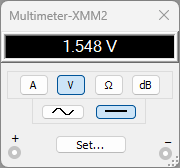
\includegraphics[width=0.48\textwidth]{Exercise1Ub.png}\hfill
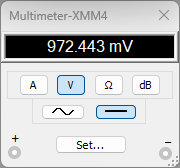
\includegraphics[width=0.48\textwidth]{Exercise1Ue.png}
\caption{Измеренные напряжения $U_\text{Б}$ и $U_\text{Э}$}
\end{figure}

\begin{equation*}
	\begin{aligned}
		U_\text{БЭ} &= U_\text{Б} - U_\text{Э} = \quad & U_\text{Б} &= \Ub \text{ В} \\
		&= \Ub - \Ue = \quad & U_\text{Э} &= \CalcThree{\Ue * 10^3} \text{ мВ} \\
		&= \Ube \text{ В}
	\end{aligned}
\end{equation*}

Снимаем с мультиметра XMMM3 показания эмиттерного тока $I_\text{Э}$.

\begin{figure}[H]
\centering
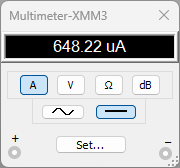
\includegraphics[width=0.48\textwidth]{Exercise1Ik.png}
\caption{Измеренный эмиттерный ток $I_\text{Э}$}
\end{figure}

\begin{equation*}
	\begin{aligned}
		U_\text{КЭ} &= U_{V1} - I_\text{К} R_6 - U_\text{Э} = \quad & I_\text{К} = \CalcThree{\Ik * 10^6} \text{ мкА} \\
		&= \Uone - \Ik \cdot 3300 - \Ue = \quad \\
		&= \Uke \text{ В}
	\end{aligned}
\end{equation*}

\begin{figure}[H]
\centering
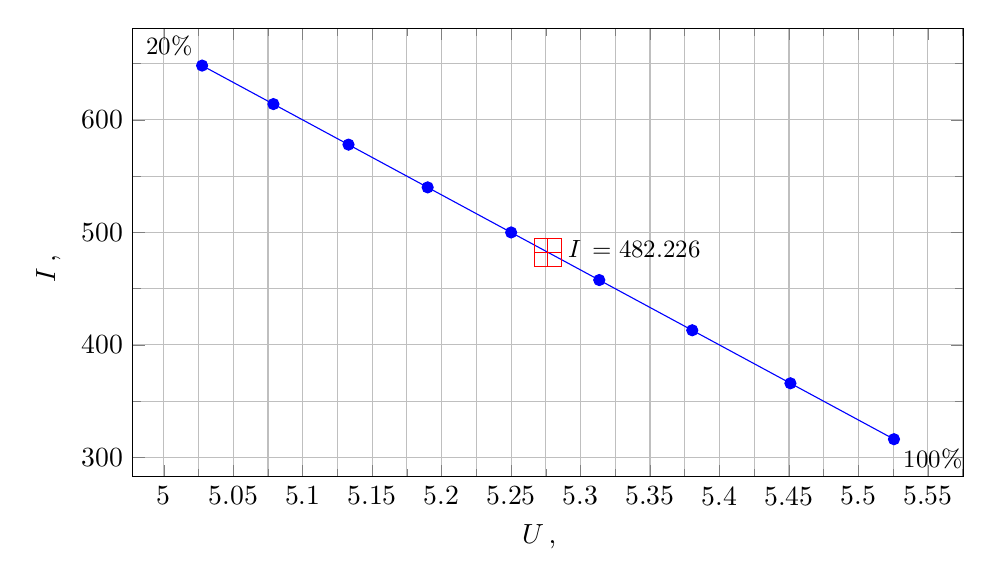
\begin{tikzpicture}
\begin{axis}[
	width=\textwidth,
	height=0.6\textwidth,
	xlabel={$U_\text{П}$, В},
	ylabel={$I_\text{К}$, мкА},
	grid=both,
	minor tick num=1,
	legend pos=north west
]
\addplot[color=blue,mark=*] coordinates {
	(\UpTwenty, \IkTwenty * 10^6)
	(\UpThirty, \IkThirty * 10^6)
	(\UpForty, \IkForty * 10^6)
	(\UpFifty, \IkFifty * 10^6)
	(\UpSixty, \IkSixty * 10^6)
	(\UpSeventy, \IkSeventy * 10^6)
	(\UpEighty, \IkEighty * 10^6)
	(\UpNinety, \IkNinety * 10^6)
	(\UpHundred, \IkHundred * 10^6)
};
\addplot[color=red,mark=square,mark size=5pt] coordinates {
	((\UpHundred + \UpTwenty) / 2, \fpeval{(\IkHundred + \IkTwenty) * 10^6 / 2})
};
\addplot[color=red,mark=|,mark size=5pt] coordinates {
	((\UpHundred + \UpTwenty) / 2, \fpeval{(\IkHundred + \IkTwenty) * 10^6 / 2})
};
\addplot[color=red,mark=-,mark size=5pt] coordinates {
	((\UpHundred + \UpTwenty) / 2, \fpeval{(\IkHundred + \IkTwenty) * 10^6 / 2})
};
\node at (axis cs:\UpTwenty, \IkTwenty * 10^6) [anchor=south east] {\small $20$\%};
\node at (axis cs:\fpeval{(\UpHundred + \UpTwenty) / 2}, \fpeval{(\IkHundred + \IkTwenty) * 10^6 / 2}) [anchor=south west,yshift=5pt,xshift=-15pt] {\small Рабочая точка};
\node at (axis cs:\fpeval{(\UpHundred + \UpTwenty) / 2}, \fpeval{(\IkHundred + \IkTwenty) * 10^6 / 2}) [anchor=west,yshift=0pt,xshift=4pt] {\small $I_\text{К} = \fpeval{(\IkHundred + \IkTwenty) * 10^6 / 2}$ мкА};
\node at (axis cs:\UpHundred, \IkHundred * 10^6) [anchor=north west] {\small $100$\%};
\end{axis}
\end{tikzpicture}
\caption{Зависимость $I_\text{К}$ от $U_\text{П}$ в усилительном каскаде}
\label{fig:exercise1Ik}
\end{figure}

\noindent\begin{minipage}{\textwidth}
	\begin{minipage}{0.48\textwidth}
		$\quad$Снимем значения $I_\text{К}$ и $U_\text{Э}$ при различных положениях переменного резистора $R_5$,
		также вычислим напряжение 
		
		\begin{equation*}
			U_\text{П} = U_{V1} - U_\text{Э}
		\end{equation*}
		
		в каждой точке. Результаты занесём в таблицу. По ней же построим график зависимости

		\begin{equation*}
			I_\text{К} = f(U_\text{П})
		\end{equation*}

		на Рис.~\ref{fig:exercise1Ik}. 

		\vspace{0.5em}

		\begin{tabularx}{\textwidth}{|C|C|p{3.2cm}|}
		\hline
		$I_\text{К}$, мкА  & $U_\text{Э}$, мВ & $U_\text{П}=U_{V1} - U_\text{Э}$, В 
		\tabularnewline
		\hline
		$\CalcThree{\IkTwenty * 10^6}$ & $\CalcThree{\UeTwenty * 10^3}$ & \centering $\CalcFive{\UpTwenty}$ 
		\tabularnewline
		$\CalcThree{\IkThirty * 10^6}$ & $\CalcThree{\UeThirty * 10^3}$ & \centering $\CalcFive{\UpThirty}$
		\tabularnewline
		$\CalcThree{\IkForty * 10^6}$ & $\CalcThree{\UeForty * 10^3}$ & \centering $\CalcFive{\UpForty}$ 
		\tabularnewline
		$\CalcThree{\IkFifty * 10^6}$ & $\CalcThree{\UeFifty * 10^3}$ & \centering $\CalcFive{\UpFifty}$ 
		\tabularnewline
		$\CalcThree{\IkSixty * 10^6}$ & $\CalcThree{\UeSixty * 10^3}$ & \centering $\CalcFive{\UpSixty}$ 
		\tabularnewline
		$\CalcThree{\IkSeventy * 10^6}$ & $\CalcThree{\UeSeventy * 10^3}$ & \centering $\CalcFive{\UpSeventy}$ 
		\tabularnewline
		$\CalcThree{\IkEighty * 10^6}$ & $\CalcThree{\UeEighty * 10^3}$ & \centering $\CalcFive{\UpEighty}$ 
		\tabularnewline
		$\CalcThree{\IkNinety * 10^6}$ & $\CalcThree{\UeNinety * 10^3}$ & \centering $\CalcFive{\UpNinety}$ 
		\tabularnewline
		$\CalcThree{\IkHundred * 10^6}$ & $\CalcThree{\UeHundred * 10^3}$ & \centering $\CalcFive{\UpHundred}$
		\tabularnewline
		\hline
		\end{tabularx}
	\end{minipage}
	\hspace{0.03\textwidth}
	\begin{minipage}{0.5\textwidth}
		\centering
		\begin{minipage}{0.42\textwidth}
			\centering
			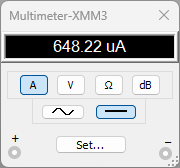
\includegraphics[width=\textwidth]{Exercise1Ik.png}
			\captionof{figure}{\small $I_\text{К}$ при $20$\%}
		\end{minipage} \hspace{0.09\textwidth}
		\begin{minipage}{0.42\textwidth}
			\centering
			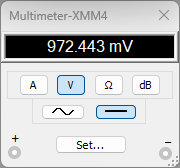
\includegraphics[width=\textwidth]{Exercise1Ue.png}
			\captionof{figure}{\small $U_\text{Э}$ при $20$\%}
		\end{minipage}
		\begin{minipage}{0.42\textwidth}
			\centering
			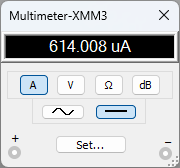
\includegraphics[width=\textwidth]{Exercise1Ik30p.png}
			\captionof{figure}{\small $I_\text{К}$ при $30$\%}
		\end{minipage} \hspace{0.09\textwidth}
		\begin{minipage}{0.42\textwidth}
			\centering
			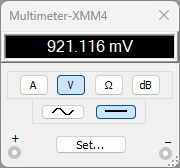
\includegraphics[width=\textwidth]{Exercise1Ue30p.png}
			\captionof{figure}{\small $U_\text{Э}$ при $30$\%}
		\end{minipage}
		\begin{minipage}{0.42\textwidth}
			\centering
			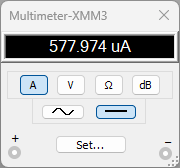
\includegraphics[width=\textwidth]{Exercise1Ik40p.png}
			\captionof{figure}{\small $I_\text{К}$ при $40$\%}
		\end{minipage} \hspace{0.09\textwidth}
		\begin{minipage}{0.42\textwidth}
			\centering
			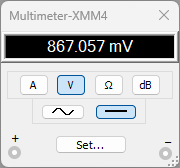
\includegraphics[width=\textwidth]{Exercise1Ue40p.png}
			\captionof{figure}{\small $U_\text{Э}$ при $40$\%}
		\end{minipage}
	\end{minipage}

	\vspace{0.5em}

	\begin{minipage}{\textwidth}
		\begin{minipage}{0.21\textwidth}
			\centering
			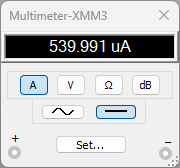
\includegraphics[width=\textwidth]{Exercise1Ik50p.png}
			\captionof{figure}{\small $I_\text{К}$ при $50$\%}
		\end{minipage} \hspace{0.045\textwidth}
		\begin{minipage}{0.21\textwidth}
			\centering
			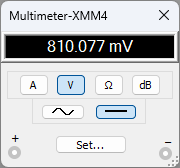
\includegraphics[width=\textwidth]{Exercise1Ue50p.png}
			\captionof{figure}{\small $U_\text{Э}$ при $50$\%}
		\end{minipage} \hspace{0.045\textwidth}
		\begin{minipage}{0.21\textwidth}
			\centering
			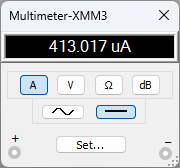
\includegraphics[width=\textwidth]{Exercise1Ik80p.png}
			\captionof{figure}{\small $I_\text{К}$ при $80$\%}
		\end{minipage} \hspace{0.045\textwidth}
		\begin{minipage}{0.21\textwidth}
			\centering
			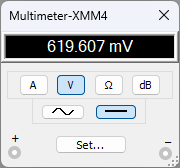
\includegraphics[width=\textwidth]{Exercise1Ue80p.png}
			\captionof{figure}{\small $U_\text{Э}$ при $80$\%}
		\end{minipage} \hspace{0.045\textwidth}
		\begin{minipage}{0.21\textwidth}
			\centering
			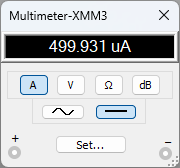
\includegraphics[width=\textwidth]{Exercise1Ik60p.png}
			\captionof{figure}{\small $I_\text{К}$ при $60$\%}
		\end{minipage} \hspace{0.045\textwidth}
		\begin{minipage}{0.21\textwidth}
			\centering
			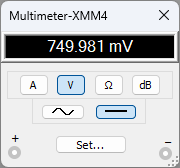
\includegraphics[width=\textwidth]{Exercise1Ue60p.png}
			\captionof{figure}{\small $U_\text{Э}$ при $60$\%}
		\end{minipage} \hspace{0.045\textwidth}
			\begin{minipage}{0.21\textwidth}
			\centering
			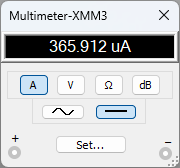
\includegraphics[width=\textwidth]{Exercise1Ik90p.png}
			\captionof{figure}{\small $I_\text{К}$ при $90$\%}
		\end{minipage} \hspace{0.045\textwidth}
		\begin{minipage}{0.21\textwidth}
			\centering
			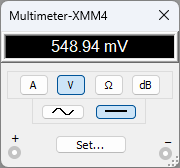
\includegraphics[width=\textwidth]{Exercise1Ue90p.png}
			\captionof{figure}{\small $U_\text{Э}$ при $90$\%}
		\end{minipage} \hspace{0.045\textwidth}
		\begin{minipage}{0.21\textwidth}
			\centering
			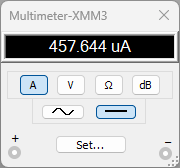
\includegraphics[width=\textwidth]{Exercise1Ik70p.png}
			\captionof{figure}{\small $I_\text{К}$ при $70$\%}
		\end{minipage} \hspace{0.045\textwidth}
		\begin{minipage}{0.21\textwidth}
			\centering
			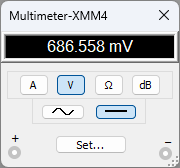
\includegraphics[width=\textwidth]{Exercise1Ue70p.png}
			\captionof{figure}{\small $U_\text{Э}$ при $70$\%}
		\end{minipage} \hspace{0.045\textwidth}
			\begin{minipage}{0.21\textwidth}
			\centering
			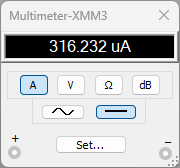
\includegraphics[width=\textwidth]{Exercise1Ik100p.png}
			\captionof{figure}{\small $I_\text{К}$ при $100$\%}
		\end{minipage} \hspace{0.045\textwidth}
		\begin{minipage}{0.21\textwidth}
			\centering
			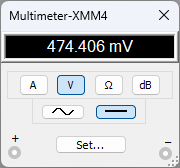
\includegraphics[width=\textwidth]{Exercise1Ue100p.png}
			\captionof{figure}{\small $U_\text{Э}$ при $100$\%}
		\end{minipage}
	\end{minipage}
\end{minipage}

Выставим сопротивление резистора $R_5 = \Rfive$ Ом, чтобы $I_\text{К} = \fpeval{(\IkHundred + \IkTwenty) * 10^6 / 2}$ мкА.


\section{Исследование усилительного каскада с ёмкостной связью по переменному току}

\fancyhead[L]{Задание $2$} 

Снимаем с мультиметра XMM1 показания действующего значения генератора $e_\text{г}$, с мультиметра 
XMM2 показания входного напряжения $U_\text{вх}$, а с мультиметра XMM5 показания выходного 
напряжения $U_\text{вых}$ для каждой амплитуды генератора $E_\text{г}$. Результаты занесём в таблицу.

\vspace{1em}

\noindent\begin{tabularx}{\textwidth}{|p{3cm}|C|C|C|C|C|C|C|C|C|C|C|C|}
	\hline
	\small $E_\text{г}$, мВ & \small $\fpeval{\EgOne * 10^3}$ & \small $\fpeval{\EgTwo * 10^3}$ & \small $\fpeval{\EgThree * 10^3}$ & 
	\small $\fpeval{\EgFour * 10^3}$ & \small $\fpeval{\EgFive * 10^3}$ \\ 
	\hline
	\small $e_\text{г}$, мВ & \small $\fpeval{\egOne * 10^3}$ & \small $\fpeval{\egTwo * 10^3}$ & \small $\fpeval{\egThree * 10^3}$ & 
	\small $\fpeval{\egFour * 10^3}$ & \small $\fpeval{\egFive * 10^3}$ \\
	\cline{1-1}
	\small $U_\text{вх}$, мВ & \small $\fpeval{\UinOne * 10^3}$ & \small $\fpeval{\UinTwo * 10^3}$ & \small $\fpeval{\UinThree * 10^3}$ & 
	\small $\fpeval{\UinFour * 10^3}$ & \small $\fpeval{\UinFive * 10^3}$ \\
	\cline{1-1}
	\small $U_\text{вых}$, мВ ($1$ кОм) & \small $\fpeval{\UoutOnekOhmOne * 10^3}$ & \small $\fpeval{\UoutOnekOhmTwo * 10^3}$ & \small $\fpeval{\UoutOnekOhmThree * 10^3}$ &
	\small $\fpeval{\UoutOnekOhmFour * 10^3}$ & \small $\fpeval{\UoutOnekOhmFive * 10^3}$ \\
	\cline{1-1}
	\small $U_\text{вых}$, мВ ($10$ кОм) & \small $\fpeval{\UoutTenkOhmOne * 10^3}$ & \small $\fpeval{\UoutTenkOhmTwo * 10^3}$ & \small $\fpeval{\UoutTenkOhmThree * 10^3}$ & 
	\small $\fpeval{\UoutTenkOhmFour * 10^3}$ & \small $\fpeval{\UoutTenkOhmFive * 10^3}$ \\
	\hline
	\small $E_\text{г}$, мВ & \small $\fpeval{\EgSix * 10^3}$ & 
	\small $\fpeval{\EgSeven * 10^3}$ & \small $\fpeval{\EgEight * 10^3}$ & \small $\fpeval{\EgNine * 10^3}$ & 
	\small $\fpeval{\EgTen * 10^3}$ \\ 
	\hline
	\small $e_\text{г}$, мВ & \small $\fpeval{\egSix * 10^3}$ & \small $\fpeval{\egSeven * 10^3}$ & 
	\small $\fpeval{\egEight * 10^3}$ & \small $\fpeval{\egNine * 10^3}$ & \small $\fpeval{\egTen * 10^3}$ \\
	\cline{1-1}
	\small $U_\text{вх}$, мВ & \small $\fpeval{\UinSix * 10^3}$ & \small $\fpeval{\UinSeven * 10^3}$ & \small $\fpeval{\UinEight * 10^3}$ & 
	\small $\fpeval{\UinNine * 10^3}$ & \small $\fpeval{\UinTen * 10^3}$ \\
	\cline{1-1}
	\small $U_\text{вых}$, мВ ($1$ кОм) & \small $\fpeval{\UoutOnekOhmSix * 10^3}$ & \small $\fpeval{\UoutOnekOhmSeven * 10^3}$ & \small $\fpeval{\UoutOnekOhmEight * 10^3}$ & 
	\small $\fpeval{\UoutOnekOhmNine * 10^3}$ & \small $\fpeval{\UoutOnekOhmTen * 10^3}$ \\
	\cline{1-1}
	\small $U_\text{вых}$, мВ ($10$ кОм) & \small $\fpeval{\UoutTenkOhmSix * 10^3}$ & \small $\fpeval{\UoutTenkOhmSeven * 10^3}$ & \small $\fpeval{\UoutTenkOhmEight * 10^3}$ & 
	\small $\fpeval{\UoutTenkOhmNine * 10^3}$ & \small $\fpeval{\UoutTenkOhmTen * 10^3}$ \\
	\hline
\end{tabularx}

\vspace{1em}

Построим амплитудную характеристику для напряжения выхода
\begin{equation*}
	U_\text{вых} = f(e_\text{г})
\end{equation*}

\begin{figure}[H]
\centering
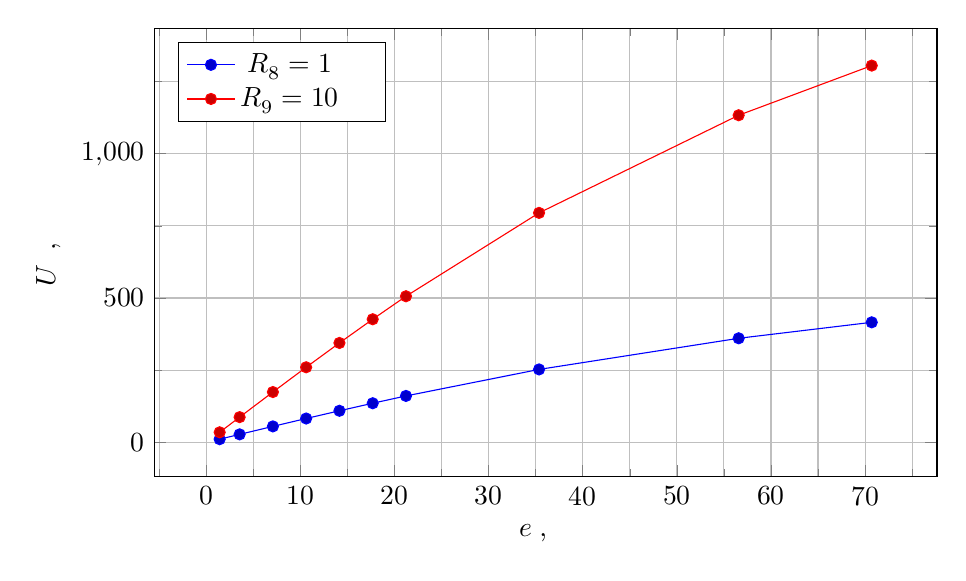
\begin{tikzpicture}
\begin{axis}[
	width=0.95\textwidth,
	height=0.6\textwidth,
	xlabel={$e_\text{г}$, мВ},
	ylabel={$U_\text{вых}$, мВ},
	grid=both,
	minor tick num=1,
	legend pos=north west
]
\addplot+[color=blue,mark=*] coordinates {
	(\egOne * 10^3, \UoutOnekOhmOne * 10^3)
	(\egTwo * 10^3, \UoutOnekOhmTwo * 10^3)
	(\egThree * 10^3, \UoutOnekOhmThree * 10^3)
	(\egFour * 10^3, \UoutOnekOhmFour * 10^3)
	(\egFive * 10^3, \UoutOnekOhmFive * 10^3)
	(\egSix * 10^3, \UoutOnekOhmSix * 10^3)
	(\egSeven * 10^3, \UoutOnekOhmSeven * 10^3)
	(\egEight * 10^3, \UoutOnekOhmEight * 10^3)
	(\egNine * 10^3, \UoutOnekOhmNine * 10^3)
	(\egTen * 10^3, \UoutOnekOhmTen * 10^3)
};
\addplot+[color=red,mark=*] coordinates {
	(\egOne * 10^3, \UoutTenkOhmOne * 10^3)
	(\egTwo * 10^3, \UoutTenkOhmTwo * 10^3)
	(\egThree * 10^3, \UoutTenkOhmThree * 10^3)
	(\egFour * 10^3, \UoutTenkOhmFour * 10^3)
	(\egFive * 10^3, \UoutTenkOhmFive * 10^3)
	(\egSix * 10^3, \UoutTenkOhmSix * 10^3)
	(\egSeven * 10^3, \UoutTenkOhmSeven * 10^3)
	(\egEight * 10^3, \UoutTenkOhmEight * 10^3)
	(\egNine * 10^3, \UoutTenkOhmNine * 10^3)
	(\egTen * 10^3, \UoutTenkOhmTen * 10^3)
};
\addlegendentry{$R_8 = 1$ кОм}
\addlegendentry{$R_9 = 10$ кОм}
\end{axis}
\end{tikzpicture}
\caption{Зависимость $U_\text{вых}$ от $e_\text{г}$ в усилительном каскаде}
\label{fig:exercise1Uout}
\end{figure}

Коэффициент усиления каскада 

\def\K{\fpeval{\UoutTenkOhmThree / \egThree}}

\begin{equation*}
	K = \frac{U_\text{вых}}{e_\text{г}} = \frac{\UoutTenkOhmThree}{\egThree} = \CalcThree{\K}
\end{equation*}
при нагрузке $R_9 = 10$ кОм, сопротивлении генератора $R_1 = 1$ кОм и амплитуде входного сигнала $E_\text{г} = 10$ мВ.

\def\rin{\fpeval{1000 / (\egFour / \UinFour - 1)}}

Входное сопротивление усилителя
\begin{equation*}
	r_\text{вх} = \frac{U_\text{вх}}{I_\text{вх}} = \frac{U_\text{вх} R_1}{e_\text{г} - U_\text{вх}} = \frac{R_1}{\frac{e_\text{г}}{U_\text{вх}} - 1} = \frac{1000}{\frac{\egFour}{\UinFour} - 1} = \CalcFour{\rin * 10^(-3)} \text{ кОм}
\end{equation*}
при нагрузке $R_9 = 10$ кОм, сопротивлении генератора $R_1 = 1$ кОм и амплитуде входного сигнала $E_\text{г} = 15$ мВ.

\def\rout{\fpeval{(\UoutTenkOhmThree - \UoutOnekOhmThree) / (\UoutOnekOhmThree / 1000 - \UoutTenkOhmThree / 10000)}}

Выходное сопротивление усилителя
\begin{equation*}
	r_\text{вых} = \frac{U_\text{вых2} - U_\text{вых1}}{\frac{U_\text{вых1}}{R_8} - \frac{U_\text{вых2}}{R_9}} = \frac{\UoutTenkOhmThree - \UoutOnekOhmThree}{\frac{\UoutOnekOhmThree}{1000} - \frac{\UoutTenkOhmThree}{10000}} = \CalcFive{\rout * 10^(-3)} \text{ кОм}
\end{equation*}
при нагрузке $R_9 = 10$ кОм и напряжении выхода $U_\text{вых2} = \fpeval{\UoutTenkOhmThree * 10^3}$ мВ и $R_8 = 1$ кОм и напряжении выхода $U_\text{вых1} = \fpeval{\UoutOnekOhmThree * 10^3}$ мВ, сопротивлении генератора $R_1 = 1$ кОм и амплитуде входного сигнала $E_\text{г} = 10$ мВ.

\section{Исследование частотных свойств усилителя}

\fancyhead[L]{Задание $3$}

Высталяем ключи в положение, в котором ток 
пройдёт через резистор $R_1$, $R_8$, конденсатор $C_3$ и не пройдёт через конденсатор $C_5$. Используем боде плоттер XBP1
для построения амплитудно-частотной характеристики усилительного каскада.

Значение $K_v$ находим для $1$ кГц
\begin{figure}[H]
\centering
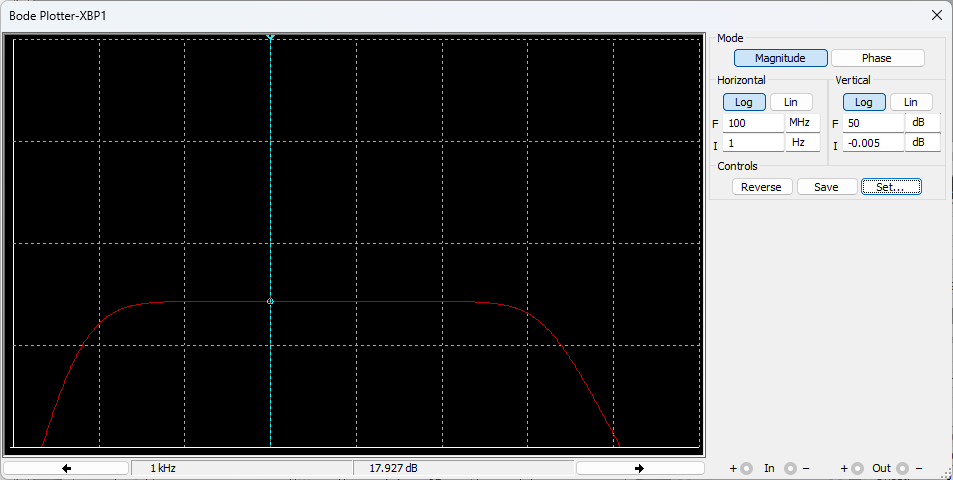
\includegraphics[width=\textwidth]{Exercise3Kv.png}
\caption{Амплитудно-частотная характеристика усилительного каскада со значением $K_v$ при $1$ кГц}
\end{figure}
после находим $f_\text{Н}$ сместив точку на $-3$ дБ от $K_v$ в сторону низких частот
\begin{figure}[H]
\centering
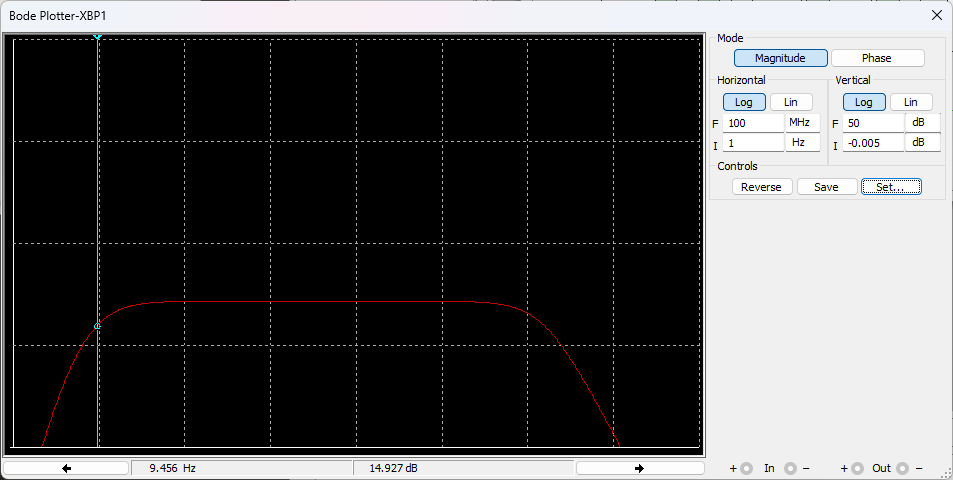
\includegraphics[width=\textwidth]{Exercise3fd.png}
\caption{Амплитудно-частотная характеристика усилительного каскада со значением $f_\text{Н}$}
\end{figure}
в завершении находим $f_\text{В}$, сместив точку на $-3$ дБ от $K_v$ в сторону высоких частот.
\begin{figure}[H]
\centering
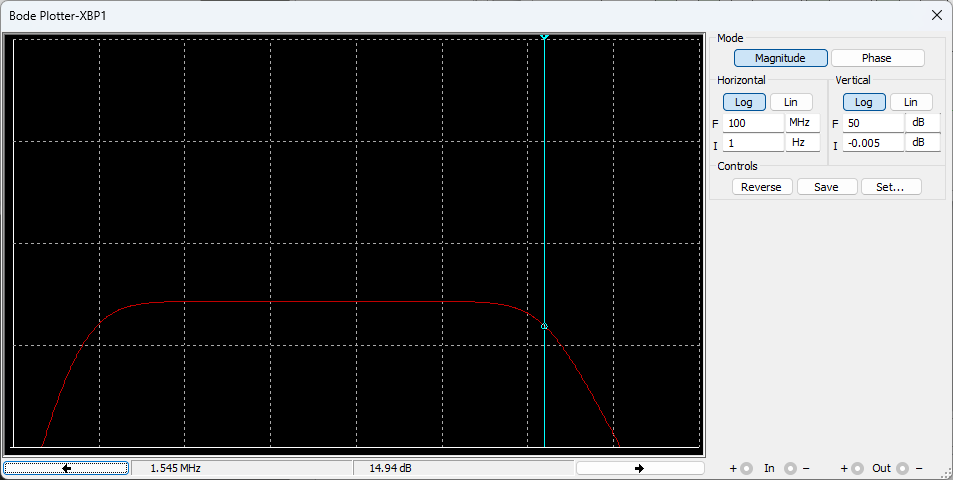
\includegraphics[width=\textwidth]{Exercise3fu.png}
\caption{Амплитудно-частотная характеристика усилительного каскада со значением $f_\text{В}$}
\end{figure}
Получаем значения $K_v = \KvOne$, $f_\text{Н} = \fpeval{\fdOne}$ Гц и $f_\text{В} = \fpeval{\fuOne / 10^6}$ 
МГц для первой конфигурации ключей. Аналогично измерение проводится для последующих конфигураций ключей.

\begin{table}[H]
	\begin{tabularx}{\textwidth}{|C|C|C|C|C|C|C|C|}
		\hline
		 & $C_\text{К}$ & $R_\text{г}$ & $R_\text{н}$ & $C_\text{н}$ & $F_\text{Н}$, Гц & $F_\text{В}$, кГц & $K_v$, dB \\
		\hline
		$1$ & $C_3$ & $R_1$ & $R_8$ & $-$ & $\fpeval{\fdOne}$ & $\fpeval{\fuOne / 10^3}$  & $\KvOne$ \\
		\cline{1-5}
		$2$ & $C_4$ & $R_1$ & $R_8$ & $-$ & $\fpeval{\fdTwo}$ & $\fpeval{\fuTwo / 10^3}$  & $\KvTwo$ \\
		\cline{1-5}
		$3$ & $C_3$ & $R_2$ & $R_8$ & $-$ & $\fpeval{\fdThree}$ & $\fpeval{\fuThree / 10^3}$  & $\KvThree$ \\
		\cline{1-5}
		$4$ & $C_3$ & $R_1$ & $R_9$ & $-$ & $\fpeval{\fdFour}$ & $\fpeval{\fuFour / 10^3}$  & $\KvFour$ \\
		\cline{1-5}
		$5$ & $C_3$ & $R_1$ & $R_8$ & $C_5$ & $\fpeval{\fdFive}$ & $\fpeval{\fuFive / 10^3}$  & $\KvFive$ \\
		\hline
	\end{tabularx}
\end{table}

Как видно из таблицы, при замене конденсатора $C_3$ на $C_4$ заметно увеличивается нижняя 
граничная частота $f_\text{Н}$, а коэффициент усиления $K_v$ и верхняя граничная частота $f_\text{В}$ не изменяются. При замене резистора $R_1$ на $R_2$ верхняя 
граничная частота $f_\text{В}$ уменьшается, как и коэффициент усиления $K_v$, происходит смещение графика вниз. 
При замене резистора $R_8$ на $R_9$ верхняя граничная частота $f_\text{В}$ уменьшается, а коэффициент 
усиления $K_v$ возрастает, график смещается вверх и левее с сужением. При добавлении конденсатора $C_5$ верхняя граничная частота $f_\text{В}$ 
заметно снижается, а коэффициент усиления $K_v$ и нижняя граничная частота $f_\text{Н}$ не изменяются.

\section{Вывод}

\fancyhead[L]{Вывод}

Определён режим работы транзистора в усилительном каскаде по постоянному току, найденый ток

\begin{equation*}
	I_\text{К} = \fpeval{(\IkHundred + \IkTwenty) * 10^6 / 2} \text{ мкА}
\end{equation*}

Проанализированы параметры усилительного каскада, такие как коэффициент усиления, входное и выходное 
сопротивление 

\begin{equation*}
	\begin{aligned}
		K &= \frac{U_\text{вых}}{e_\text{г}} = \CalcThree{\K} \\
		r_\text{вх} &= \frac{U_\text{вх}}{I_\text{вх}} = \CalcFour{\rin * 10^(-3)} \text{ кОм} \\
		r_\text{вых} &= \frac{U_\text{вых2} - U_\text{вых1}}{\frac{U_\text{вых1}}{R_8} - \frac{U_\text{вых2}}{R_9}} = \CalcFour{\rout * 10^(-3)} \text{ кОм}
	\end{aligned}
\end{equation*}
при $R_\text{г}=R_1=1$ кОм и переменном $R_\text{н}$ и $E_\text{г}$.

Из анализа частотных свойств усилителя можно сделать вывод, что замена конденсатора регулирует пропускаемые частоты, притом в зависимости от 
того, меняется конденсатор в цепи коллектора или в цепи эмиттера, изменяется нижняя или верхняя граничная
частота соответственно. Замена резистора изменяет коэффициент усиления сдвигом графика.

\end{document}